\section{Thiết kế giao diện người dùng}

Phần này trình bày thiết kế giao diện người dùng cho hệ thống E-commerce, tập trung vào các màn hình chính và cách tích hợp chức năng gợi ý sản phẩm vào trải nghiệm mua sắm. Thiết kế tuân theo nguyên tắc đặt người dùng làm trung tâm (User-Centered Design) và đảm bảo tính nhất quán trên các thiết bị.

\subsection{Nguyên tắc thiết kế}

Giao diện người dùng được xây dựng dựa trên bốn nguyên tắc chính. Đầu tiên là tính đơn giản: giao diện phải trực quan, dễ sử dụng ngay cả với người dùng lần đầu. Thứ hai là tính nhất quán: các thành phần UI, màu sắc, và cách tương tác phải thống nhất trên toàn bộ ứng dụng. Thứ ba là tính đáp ứng: giao diện phải hoạt động tốt trên mọi kích thước màn hình từ điện thoại di động đến màn hình máy tính. Cuối cùng là hiệu năng: thời gian tải trang và phản hồi tương tác phải nhanh để không làm gián đoạn trải nghiệm người dùng.

\subsection{Thiết kế trang chủ}

Trang chủ là điểm tiếp xúc đầu tiên của người dùng với hệ thống và đóng vai trò quan trọng trong việc thu hút sự chú ý và định hướng hành vi mua sắm.

\begin{figure}[H]
    \centering
    % Đã thay thế placeholder bằng home.jpg
    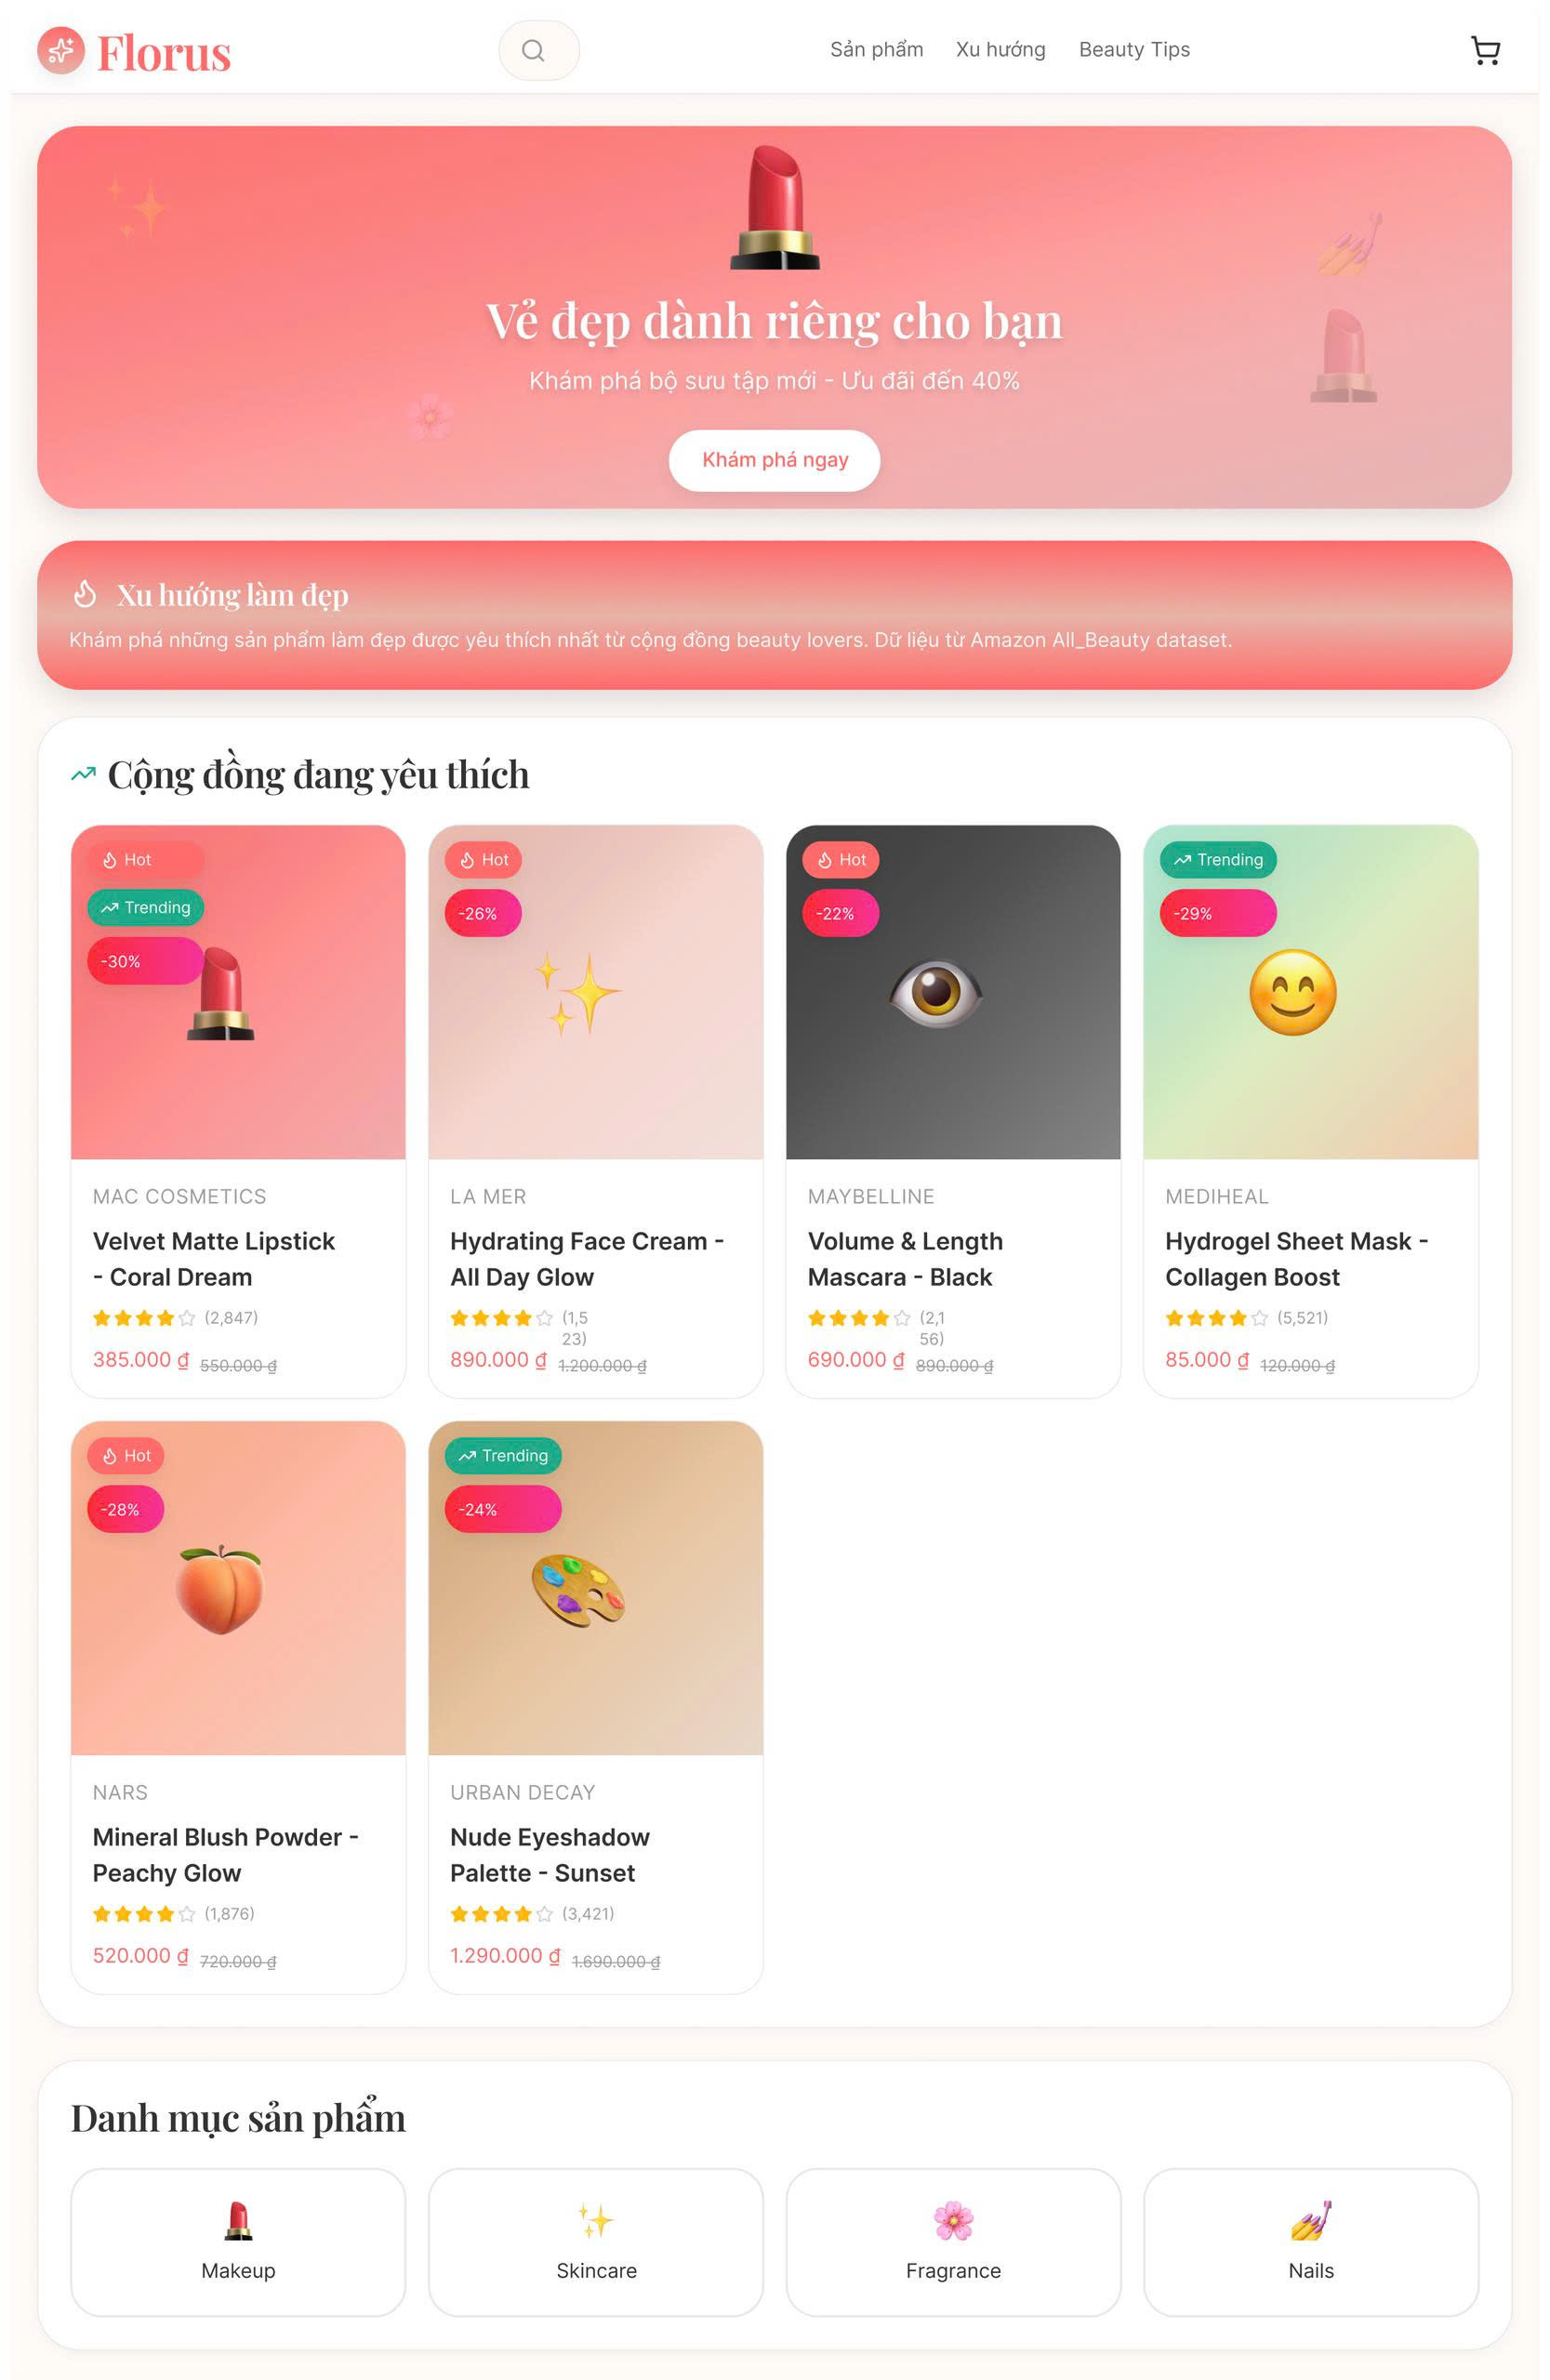
\includegraphics[width=0.6\textwidth]{images/chap 4/home.jpg}
    \vspace{0.5cm} 
    \caption{Thiết kế giao diện trang chủ}
    \label{fig:homepage-design}
\end{figure}

Trang chủ được chia thành các khu vực chức năng rõ ràng. Phần đầu trang (Header) chứa logo, thanh tìm kiếm, và các liên kết nhanh đến giỏ hàng và tài khoản người dùng. Thanh tìm kiếm được thiết kế nổi bật với tính năng gợi ý từ khóa (Autocomplete) để hỗ trợ người dùng tìm kiếm nhanh hơn.

Ngay dưới header là Banner quảng cáo dạng carousel, hiển thị các chương trình khuyến mãi và sản phẩm nổi bật. Kế tiếp là khu vực danh mục sản phẩm với các icon và hình ảnh đại diện, cho phép người dùng truy cập nhanh vào danh mục quan tâm.

Phần quan trọng nhất của trang chủ là các Widget gợi ý sản phẩm. Widget ``Sản phẩm thịnh hành'' hiển thị danh sách sản phẩm được lấy từ Popular Engine, phù hợp cho người dùng mới truy cập lần đầu. Đối với người dùng quay lại (returning users), hệ thống hiển thị thêm widget ``Dựa trên lịch sử xem của bạn'' với các sản phẩm được cá nhân hóa từ AI Model.

\subsection{Thiết kế trang chi tiết sản phẩm}

Trang chi tiết sản phẩm là nơi người dùng đưa ra quyết định mua hàng, do đó cần cung cấp đầy đủ thông tin và trình bày một cách hấp dẫn.

\begin{figure}[H]
    \centering
    % Đã thay thế placeholder bằng detail.jpg
    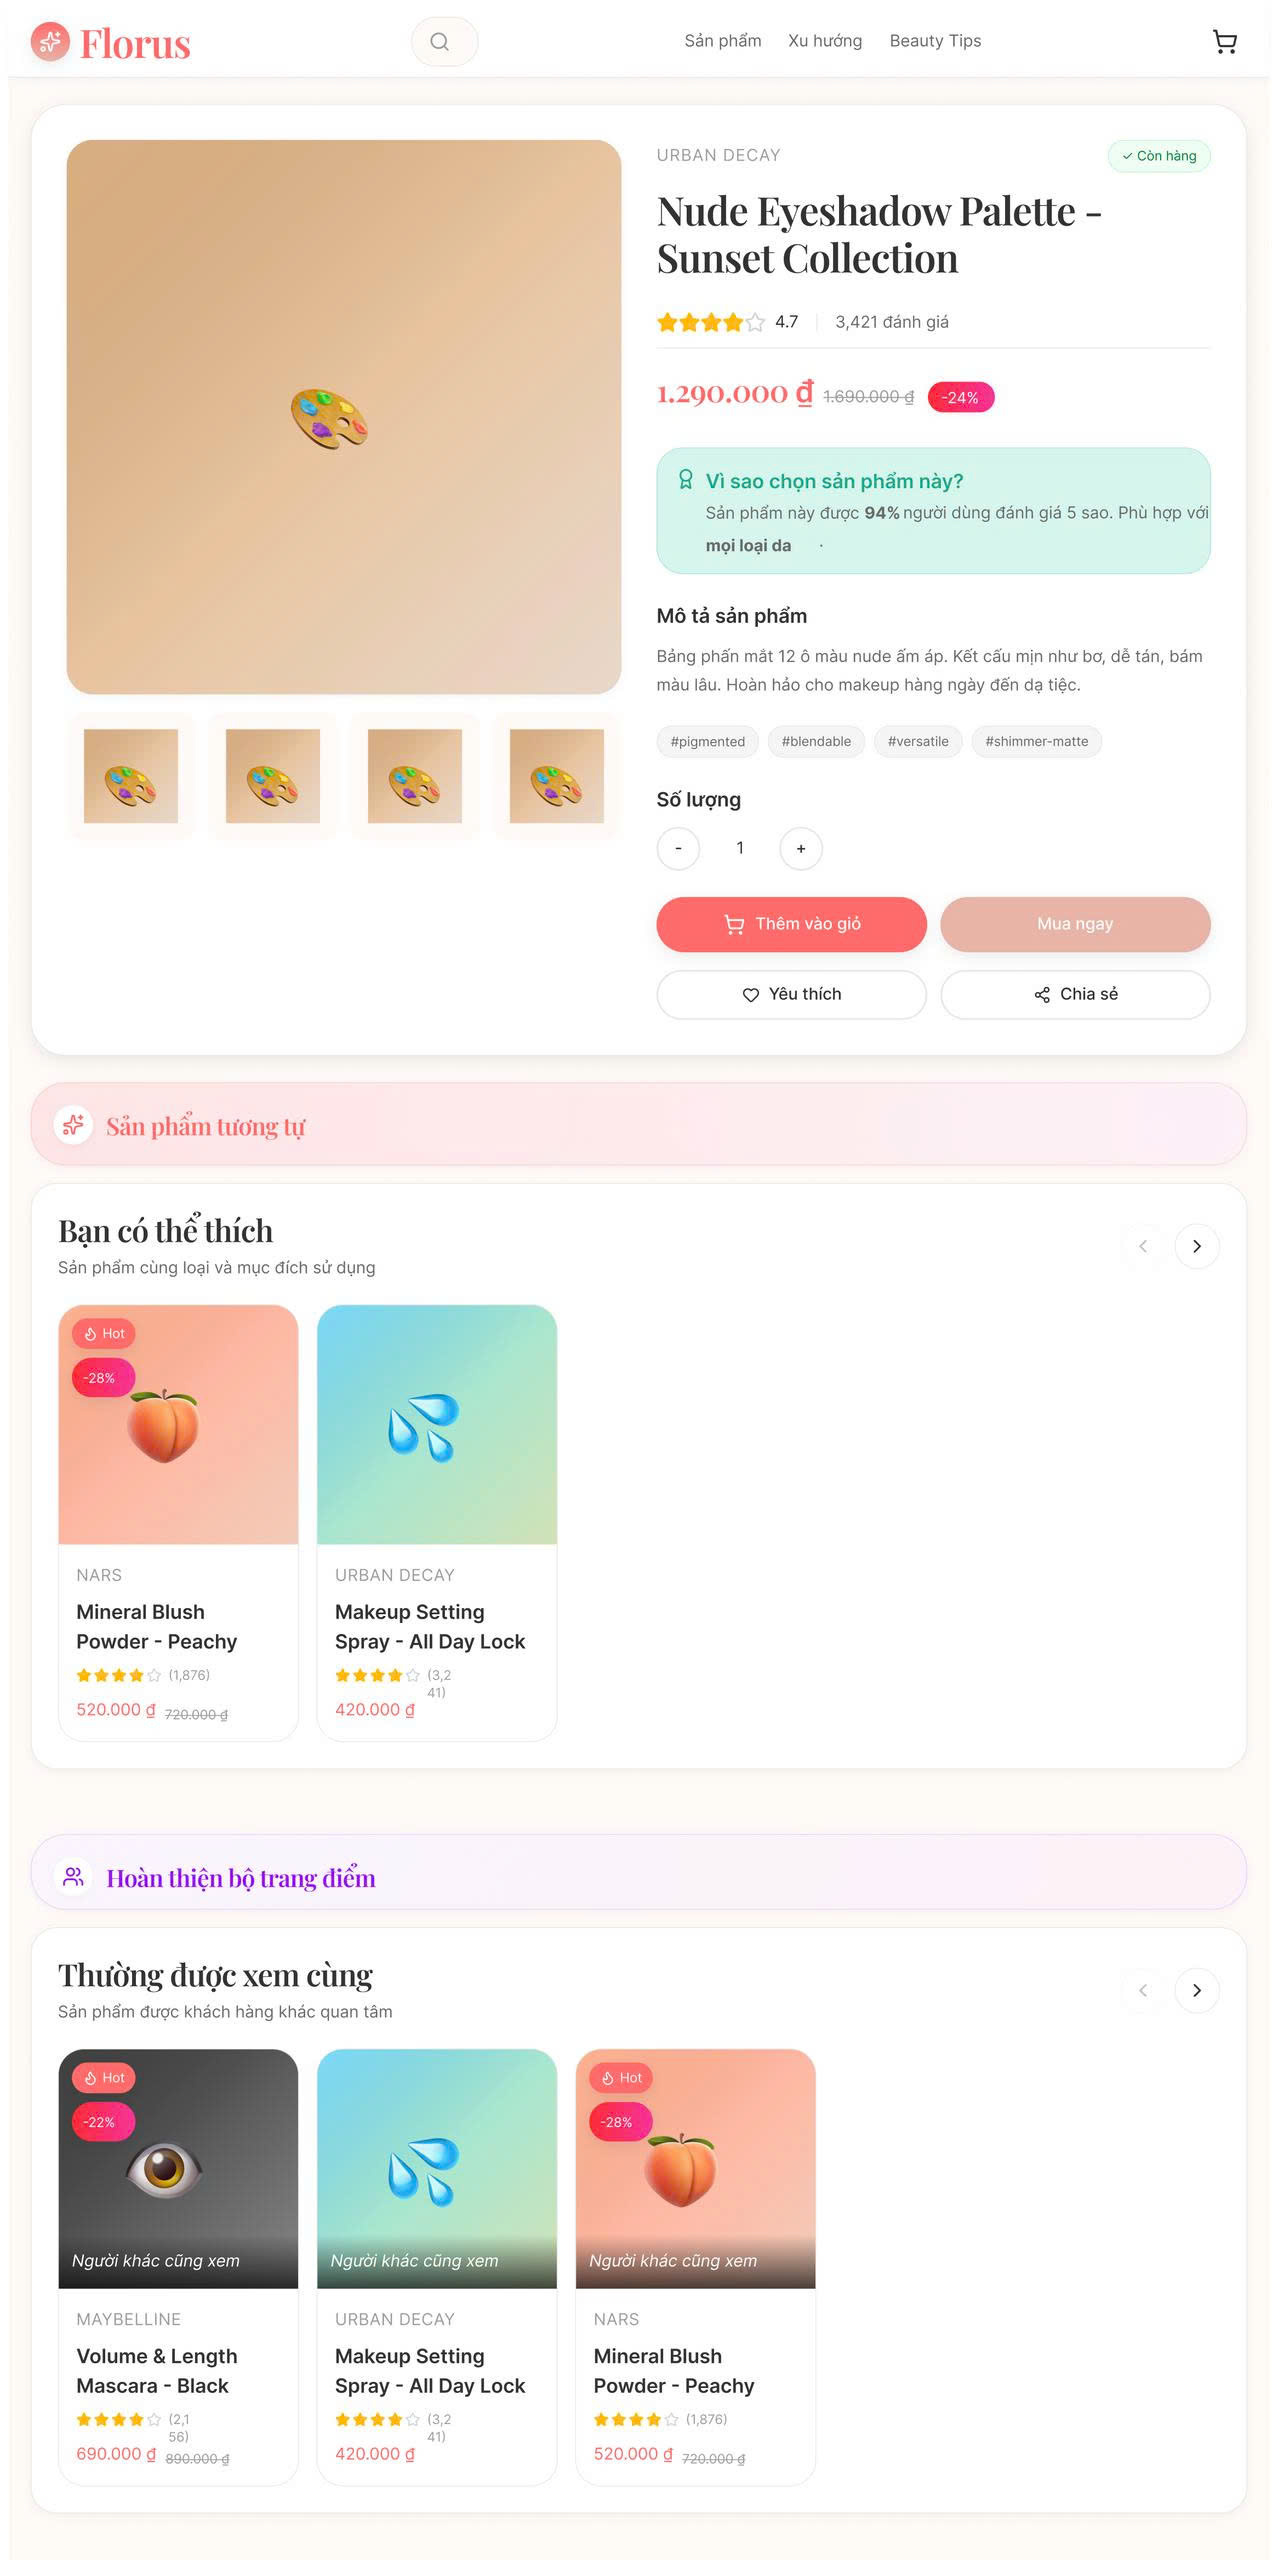
\includegraphics[width=0.6\textwidth]{images/chap 4/detail.jpg}
    \vspace{0.5cm} 
    \caption{Thiết kế giao diện trang chi tiết sản phẩm}
    \label{fig:product-detail-design}
\end{figure}

Phần trên của trang hiển thị hình ảnh sản phẩm ở kích thước lớn với khả năng zoom và xem nhiều góc. Bên cạnh là thông tin cơ bản gồm tên sản phẩm, giá (hiển thị cả giá gốc và giá khuyến mãi nếu có), đánh giá trung bình từ khách hàng, và nút ``Thêm vào giỏ hàng''.

Phần giữa trang chứa mô tả chi tiết sản phẩm, thông số kỹ thuật, và các đánh giá từ khách hàng đã mua. Tab navigation được sử dụng để tổ chức nội dung một cách gọn gàng.

Phần dưới của trang là khu vực gợi ý sản phẩm, bao gồm hai widget quan trọng. Widget ``Sản phẩm tương tự'' hiển thị các sản phẩm cùng danh mục hoặc có đặc điểm giống với sản phẩm đang xem. Widget ``Khách hàng cũng xem'' hiển thị các sản phẩm thường được xem cùng dựa trên dữ liệu CO\_VIEWED từ Neo4j. Hai widget này giúp tăng khả năng người dùng khám phá thêm sản phẩm và tăng giá trị đơn hàng trung bình.



\subsection{Thiết kế giỏ hàng và thanh toán}

Quy trình giỏ hàng và thanh toán được thiết kế đơn giản với số bước tối thiểu để giảm tỷ lệ bỏ giỏ (Cart Abandonment Rate).

\begin{figure}[H]
    \centering
    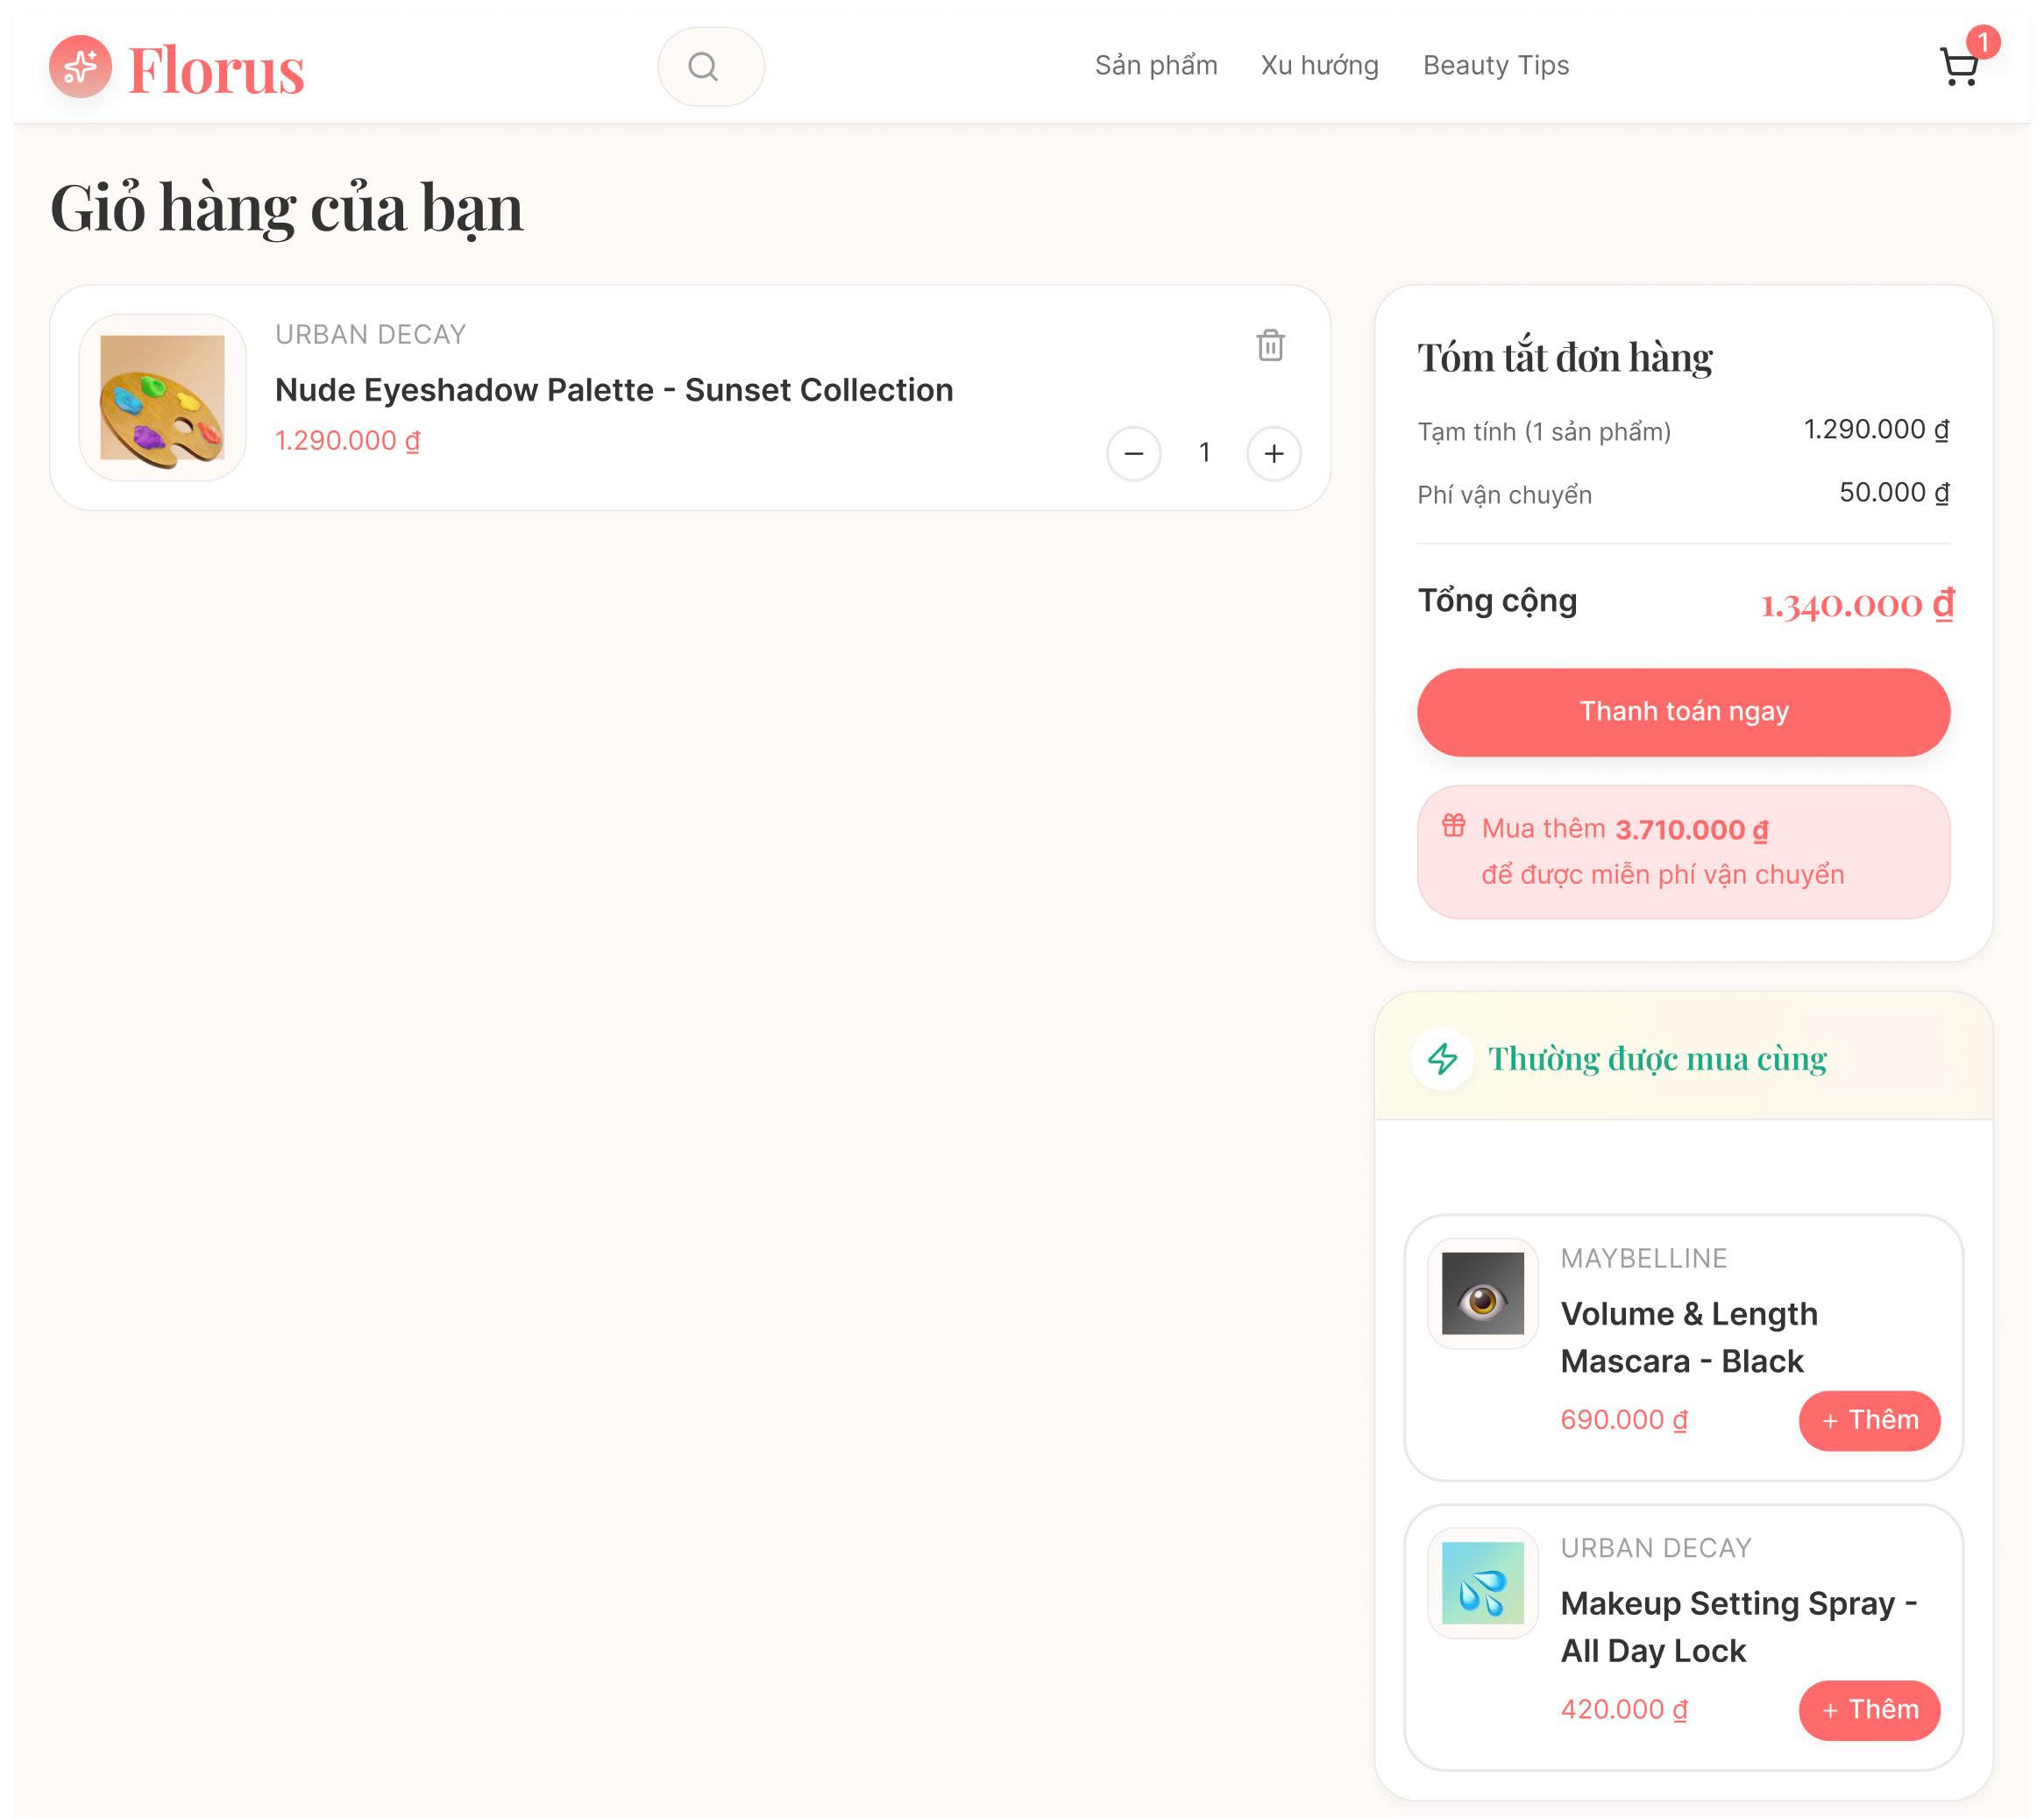
\includegraphics[width=0.9\textwidth]{images/chap 4/order.jpg}
    \vspace{0.5cm} 
    \caption{Thiết kế giao diện giỏ hàng với gợi ý Cross-sell}
    \label{fig:cart-design}
\end{figure}

Trang giỏ hàng hiển thị danh sách sản phẩm đã thêm với khả năng điều chỉnh số lượng và xóa sản phẩm. Tổng giá trị đơn hàng được cập nhật realtime khi người dùng thay đổi.

Một điểm đặc biệt trong thiết kế là tích hợp gợi ý Cross-sell ngay trong trang giỏ hàng. Widget ``Thường được mua cùng'' hiển thị các phụ kiện hoặc sản phẩm bổ sung phù hợp với những gì người dùng đang mua. Ví dụ, nếu người dùng đang mua điện thoại, widget sẽ gợi ý ốp lưng, tai nghe, hoặc sạc dự phòng. Đây là cơ hội tăng giá trị đơn hàng (Average Order Value) một cách tự nhiên.

Quy trình thanh toán được thiết kế theo dạng Single-page Checkout với các bước thu thập thông tin giao hàng, chọn phương thức thanh toán, và xác nhận đơn hàng được hiển thị trên cùng một trang. Progress indicator giúp người dùng biết họ đang ở bước nào.
